\section{Servidor na Nuvem}
Como foi escolhida uma arquitetura baseada microsserviços para construção do projeto, módulos diferentes podem ser escritos em linguagens de programação diferentes, o que promove uma maior flexibilidade não só durante o desenvolvimento dos módulos de mostrados nesse trabalho, mas também daqueles projetados futuramente como extensões do sistema Hedwig.

Para o desenvolvimento dos módulos definidos na especificação do projeto, utilizamos tecnologias atuais que são utilizadas em grandes empresas de tecnologia do mundo e possuem vasta documentação, referências e fontes de conhecimento como tutoriais e exemplos.
Para o desenvolvimento da parte de software, utilizaremos tecnologias atuais, que são também utilizadas nas maiores empresas de tecnologia do mundo. De acordo com o planejamento, utilizaremos uma arquitetura de microsserviços para construção do projeto. Com esta técnica, módulos diferentes poderiam ser escritos em, inclusive, linguagens de programação diferentes, o que promove uma maior flexibilidade durante o desenvolvimento.
Para o desenvolvimento da API, responsável pelos módulos sendo executados na nuvem e comunicação com banco de dados, utilizaremos Node.js (interpretador de código JavaScript do lado do servidor), com a utilização de alguns frameworks como é o caso do Express. O banco de dados com a qual ela se conecta é do tipo MongoDB (banco de dados orientado a documentos). Tais decisões foram baseadas no fato de bancos de dados em MongoDB serem altamente escaláveis e flexíveis, assim como Node.js, que, por sua arquitetura movida a eventos de E/S que não bloqueiam o servidor, provê ao mesmo uma altíssima escalabilidade, ao permitir milhares de conexões simultâneas, sem impacto na performance do servidor. Além disso, o fato de que os dados provindos do banco já estão organizados em objetos, e dessa forma, podem ser recebidos prontamente como objetos JavaScript no código em Node.Js geram facilidade e fluidez para o desenvolvimento do código.

\subsection{Arquitetura de Microsserviços}
\subsubsection{Características}
A arquitetura de microsserviços é um estilo que compreende a estruturação de uma aplicação em um conjunto de serviços com baixo grau de acoplamento que se comunicam por meio de protocolos de comunicação leves.

Para melhor compreender essa arquitetura, podemos compará-la à arquitetura monolítica. Uma aplicação monolítica está contida em uma única unidade, que geralmente é dividida em camadas de funcionalidade tecnológica como interface web, camada de negócios server-side e camada de persistência de dados. A escalabilidade desse modelo é dada por meio do aumento do número de servidores, máquinas virtuais ou contêineres juntamente a um load balancer - é a chamada escalabilidade horizontal. Uma alteração em uma pequena parte da aplicação significa que toda a aplicação deverá passar por um processo de \textit{build} e \textit{deploy}. Já a arquitetura de microsserviços divide as funcionalidades em serviços autônomos, muitas vezes usando as regras de negócios para realizar essa divisão. Cada serviço tem seu próprio ciclo de desenvolvimento e pode ser atualizado independentemente. A escalabilidade também é tratada serviço a serviço.

\begin{figure}[H]
	\centering
	\caption{Comparação entre uma aplicação monolítica (esquerda) e com microsserviços (direita)}
  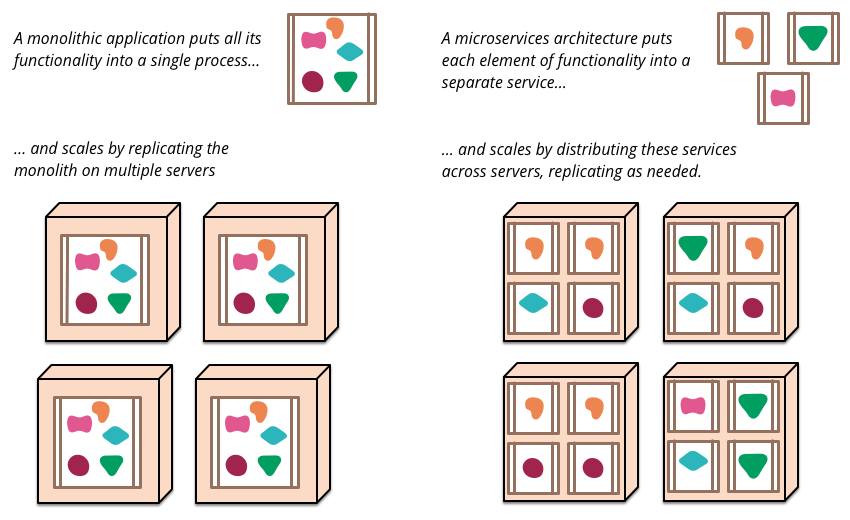
\includegraphics[width=0.8\textwidth]{estruturaMicrosservicos}
\label{fig:estruturaMicrosservicos}
\end{figure}

É difícil delimitar uma definição formal para arquitetura de microsserviços, pois não existe consenso a respeito de sua definição formal. Contudo, existe uma série de características que projetos usando essa arquitetura compartilham. Detalhamos a seguir alguns atributos e aspectos dos microsserviços. Nem todos os projetos possuem rigorosamente todas as características, mas a maioria deles possui um perfil similar ao descrito aqui.

\begin{itemize}
\item \textbf{Serviços são processos.}Pode-se fazer um mapeamento de um processo para um serviço, porém isso é apenas uma aproximação, podendo um serviço ser constituído por uma aplicação de múltiplos processos.
\item \textbf{Serviços comunicam-se por protocolos leves.}Geralmente, são usados protocolos como o HTTP.
\item \textbf{Serviços implementam capabilidades do negócio.}Isto é, a divisão de serviços é baseada nas regras de negócio e nas funcionalidades que o produto deverá suprir.
\item \textbf{Serviços são facilmente substituíveis.}
\item \textbf{Cada serviço tem um ciclo de vida independente.}Isso inclui o desenvolvimento e os processos de \textit{deploy}. Um microsserviço pode ser implementado e atualizado independentemente dos outros.
\end{itemize}

As vantagens da arquitetura de microsserviços giram em torno da modularidade e autonomia dos serviços que é natural à sua estrutura. Com isso, pode-se ter uma heterogeneidade de tecnologias, isto é, cada serviço pode ser desenvolvido usando diferentes linguagens, \textit{frameworks} e ferramentas de acordo com seus requisitos. A independência entre serviços também possibilita o deploy automatizado e o uso de práticas de integração contínua. Também há benefícios de aspecto gerencial: como cada serviço tem como escopo uma capabilidade do negócio que envolve interfaces de interação com usuário, código em várias camadas que implementa as funcionalidades necessárias e persistência em bancos de dados, é possível criar pequenas equipes multidisciplinares para cada microsserviço.

Building for failure % TODO

Existem trade-offs que devem ser considerados ao decidir pela arquitetura de microsserviços. A comunicação entre serviços por meio de uma rede possui maior latência e exige maior processamento do que mensagens trocadas a nível de processos. Por isso, é muito importante analisar as fronteiras dos serviços e a alocação de responsabilidades durante do projeto. A descentralização de dados entre microsserviços traz também a necessidade de métodos para manter a consistência das informações. Outro ponto crítico são sistemas com alta granularidade de microsserviços, causando overhead tanto de comunicação como de código além de uma fragmentação lógica que causa mais impactos negativos na complexidade e performance do que benefícios - tal caso de antipadrão foi chamado de nanosserviço \cite{rotem}.

% TODO melhorar paragrafo abaixo
Os microsserviços podem ser vistos como um estilo específico de arquitetura orientada a serviços (\textit{Service-oriented architecture} - SOA), visto que existem várias características compartilhadas entre os dois. Contudo, o termo arquitetura orientada a serviços é muito amplo, e muitas de suas implementações podem não seguir certos pontos apresentados como aspectos dos microsserviços, como por exemplo, o uso de grande inteligência no mecanismo de comunicação de dados ao invés de delegar tal complexidade aos endpoints do serviço \cite{james}. Esse e outros problemas conhecidos das experiências passadas de sistemas estruturados em SOA fazem com que muitos encarem os microsserviços como uma modernização da arquitetura orientada a serviços.

Apesar do termo microsserviço ter surgido por volta de 2011 \cite{james}, as ideias por trás desse estilo arquitetural não são recentes. O aumento da discussão em torno dos microsserviços nos últimos anos pode ser creditada a avanços tecnológicos tais como a disseminação dos serviços de nuvem, o crescimento de ferramentas de automatização de deployment, a consolidação dos conceitos de DevOps, entre outros.

\subsubsection{Casos de uso} % TODO

\subsubsection{Microsserviços e Internet das Coisas} % TODO
